\documentclass[12pt,letterpaper,final]{article}

%\documentstyle[12pt,graphicx,natbib,hyperref,Sweave,rotating]{article}

\usepackage{Sweave}
\usepackage{graphicx}
\usepackage{natbib}
\usepackage{hyperref}
\usepackage{caption}
\usepackage{rotating}
\usepackage{verbatim}
\usepackage{textcomp}

\setlength{\oddsidemargin}{0in}
\setlength{\textwidth}{6.15in}
\setlength{\topmargin}{0.5in}
\setlength{\textheight}{22cm}
\setlength{\headheight}{0in}
\setlength{\headsep}{0in}
\setlength{\parskip}{5pt plus 2pt minus 3pt}

\marginparwidth2cm
\marginparsep0.2cm
\marginparpush0.2cm
%\tabcolsep0pt

\def\thefootnote{\fnsymbol{footnote}}
\setcounter{footnote}{1}

\renewcommand{\baselinestretch}{1.2}
\renewcommand{\labelenumi}{(\roman{enumi})}

\renewcommand{\topfraction}{1.0}
\renewcommand{\bottomfraction}{1.0}
\renewcommand{\textfraction}{0.0}
\renewcommand{\floatpagefraction}{1.0}

\newtheorem{definition}{Definition}
\newtheorem{theorem}{Theorem}
\newtheorem{lemma}[theorem]{Lemma}
\newtheorem{claim}[theorem]{Claim}
\newtheorem{fact}[theorem]{Fact}

% to get nice proofs ...
\newcommand{\qedsymb}{\mbox{ }~\hfill~{\rule{2mm}{2mm}}}
\newenvironment{proof}{\begin{trivlist}
\item[\hspace{\labelsep}{\bf\noindent Proof: }]
}{\qedsymb\end{trivlist}}

\def\printindex{\input{\jobname.ind}}

\newfont{\msymb}{cmsy10 scaled 1000}

\def\nullset{\mbox{\O}}
\def\R{{I\!\!R}}
\def\N{{I\!\!N}}
\def\C{{C\!\!\!\!I}}

\def\convdist{\stackrel{d}{\longrightarrow}}
\def\convlaw{\stackrel{L}{\longrightarrow}}
\def\convweak{\stackrel{w}{\longrightarrow}}
\def\convprob{\stackrel{p}{\longrightarrow}}
\def\convmean#1{\stackrel{#1}{\longrightarrow}}
\def\convas{\stackrel{a.s.}{\longrightarrow}}
\def\convwp{\stackrel{w.p.1}{\longrightarrow}}

\def\A{\mbox{\msymb A}}
\def\B{\mbox{\msymb B}}
\def\H{\mbox{\msymb H}}
\def\P{\mbox{\msymb P}}
\def\S{\mbox{\msymb S}}
\def\X{\mbox{\msymb X}}
\def\Y{\mbox{\msymb Y}}

\def\u0{\underline{0}}
\def\ua{\underline{a}}
\def\ub{\underline{b}}
\def\ud{\underline{d}}
\def\ug{\underline{g}}
\def\ueta{\underline{\eta}}
\def\umu{\underline{\mu}}
\def\utheta{\underline{\theta}}
\def\uvartheta{\underline{\vartheta}}
\def\UT{\underline{T}}
\def\ut{\underline{t}}
\def\UU{\underline{U}}
\def\uu{\underline{u}}
\def\OX{\overline{X}}
\def\UX{\underline{X}}
\def\ux{\underline{x}}
\def\UY{\underline{Y}}
\def\uy{\underline{y}}
\def\UZ{\underline{Z}}
\def\uz{\underline{z}}

%\parskip 0.1in
\pagenumbering{arabic}    %  Start using 1,2,... as page numbers.
\pagestyle{plain}         %  Page numbers in middle bottom of page.
%\setcounter{page}{80}  % XXXXXXXXXXXXXXXXX
%\setcounter{theorem}{5} % XXXXXXXXXXXXXXXXX
%\setcounter{definition}{10} % XXXXXXXXXXXXXXXXX

\parindent 0in

\makeindex


\begin{document}

\Sconcordance{concordance:lect_main.tex:lect_main.Rnw:%
1 164 1}
\Sconcordance{concordance:lect_main.tex:./lect_acknow.Rnw:ofs 165:%
1 40 1}
\Sconcordance{concordance:lect_main.tex:lect_main.Rnw:ofs 206:%
167 13 1}
\Sconcordance{concordance:lect_main.tex:./lect_chapter6.Rnw:ofs 220:%
1 27 1 1 2 12 0 3 1 2 2 1 3 1 0 1 3 1 0 1 1 1 3 1 0 1 1 1 3 1 0 1 1 4 0 %
1 2 6 1 1 2 1 0 1 1 1 3 1 0 1 4 2 0 1 4 2 0 1 5 3 0 1 2 4 0 1 2 15 1 1 %
2 1 0 2 2 1 1 1 2 1 0 1 2 1 1 1 2 1 0 1 2 1 1 1 2 1 0 1 2 1 1 1 2 1 0 1 %
2 1 1 1 2 1 0 1 2 1 1 1 2 5 0 1 2 10 1 1 2 1 0 1 3 1 0 1 1 1 2 1 3 1 0 %
1 1 1 3 1 0 1 1 1 3 1 0 1 1 4 0 1 2 1 1 1 2 1 0 1 1 1 2 1 8 6 0 1 8 6 0 %
1 1 3 0 1 2 1 1 1 9 8 0 1 1 3 0 1 2 1 1 1 7 6 0 1 1 3 0 1 2 1 1 1 2 5 0 %
1 2 21 1 1 2 1 0 1 1 1 2 4 0 2 2 5 0 2 2 5 0 2 2 5 0 2 2 5 0 2 2 5 0 1 %
2 3 1 1 2 1 0 1 1 1 5 3 0 1 1 3 0 1 2 1 1 1 5 4 0 1 1 3 0 1 2 1 1 1 2 5 %
0 1 2 11 1 1 47 49 0 1 2 8 1 1 2 1 0 1 1 1 2 5 0 1 2 5 0 1 2 6 0 1 2 5 %
1 4 0 1 3 5 1 1 2 6 0 1 2 1 4 6 0 1 2 29 1}
\Sconcordance{concordance:lect_main.tex:lect_main.Rnw:ofs 698:%
182 28 1}



\bibliographystyle{agsm}

\begin{titlepage}
\vspace*{3.5cm}
\begin{center}
{\LARGE \bf Stat 5810, Section 005 \&} \\[0.5cm]
{\LARGE \bf Stat 6910, Section 003} \\[0.8cm]
{\LARGE \bf Statistical Visualization II} \\[0.5cm]
{\LARGE \bf Spring 2019} \\[0.5cm]
~ \\[2cm]
{\bf Dr. J\"urgen Symanzik} \\[0.3cm]
Utah State University \\[0.3cm]
Department of Mathematics and Statistics \\[0.3cm]
3900 Old Main Hill \\[0.3cm]
Logan, UT 84322--3900 \\[0.8cm]
Tel.: (435) 797--0696 \\[0.3cm]
FAX: (435) 797--1822 \\[0.3cm]
e-mail: \verb|symanzik@math.usu.edu| \\[0.3cm]
Web: \url{http://www.math.usu.edu/~symanzik/}
\end{center}

\thispagestyle{empty}
\vfill
\end{titlepage}

\newpage

\thispagestyle{empty}

\vspace*{5cm}

\begin{figure}[ht]
\centering{\includegraphics[width=0.99\textwidth]{Scans//PhdcomicsCom_Plotting.jpg}}
\caption{\label{PhdcomicsCom_Plotting}
\url{http://www.phdcomics.com/comics/archive.php?comicid=1541}, \\
Cartoon.
}
\end{figure}


\newpage


\setcounter{page}{1}

\tableofcontents

\newpage

%~
%
%\newpage

% !Rnw root = lect_main.Rnw

\section*{Acknowledgements}

This course uses some of the course materials provided by
Dr.\ Mike Minnotte (formerly USU, now with the University of
North Dakota) as held in the Fall 2006 semester. Additional materials
have been taken from other Statistical Graphics courses, such as the
ones offered by Dr.\ Di Cook (formerly Iowa State University; now Monash University:
\url{http://dicook.org/}) and
Dr.\ Dan Carr (George Mason University: \url{http://mason.gmu.edu/~dcarr/}).
Other examples and R code originate from 
David Kahle, Heike Hofmann, Carson Sievert,
Martin Theus, Antony Unwin, Simon Urbanek, Hadley Wickham, Lee Wilkinson, and others.
We are likely to include parts from additional authors and sources
that will be specified later during the semester.

Thanks are also due to 80+ students and guests who took 
the former ``Stat 6560: Graphical Methods'' and
the current ``Statistical Visualization I \& II'' courses
with me since the Spring 2009 semester 
for their valuable comments that helped
to improve, correct, and extend these lecture notes.


~\\
J\"urgen Symanzik, January 21, 2019.


\begin{figure}[ht]
\centering{\includegraphics[width=3.5in]{Scans//Zelazny_px_Fig.jpg}}
\caption{\label{Zelazny_px_Fig}
\cite{Ze2001}, p.~x, Cartoon.
}
\end{figure}

\newpage

%~\\
%
%\newpage
\addcontentsline{toc}{section}{Acknowledgements}

\newpage


\setcounter{page}{1}

%\SweaveInput{lect_chapter0.Rnw}
%\SweaveInput{unwin_chapter1IntroRgda-knitr_mod.Rnw}
%\SweaveInput{lect_chapter11.Rnw}
%\SweaveInput{lect_chapter4.Rnw}
%\SweaveInput{lect_chapter5.Rnw}
%\SweaveInput{lect_chapter1.Rnw}

% !Rnw root = lect_main.Rnw

\def\jsprivatechsix{1} % show additional details
%\def\jsprivatechsix{0} % do NOT show additional details


\section{Bivariate Plots}

%{\bf (Based on \cite{Wa97}, Chapter 1 \& \cite{Tu83}, Chapter 2)}


\subsection{Scatterplots}

\cite{WWPJH96}, p.~46, state: 
\begin{quotation}
``Scatterplots are used to show relationship (causal relationship or covariance)
between two {\it quantitative} variables. The data consists of a number of pairs
of coordinates $(x, y)$. Each pair of coordinates is indicated by a dot or circle
in a system of coordinates.''
\end{quotation}


In the next example, we resume work with 
the iris data introduced in the previous chapter.


\underline{\bf Example 1:}
%
\begin{Schunk}
\begin{Sinput}
> head(iris)
\end{Sinput}
\begin{Soutput}
  Sepal.Length Sepal.Width Petal.Length Petal.Width Species
1          5.1         3.5          1.4         0.2  setosa
2          4.9         3.0          1.4         0.2  setosa
3          4.7         3.2          1.3         0.2  setosa
4          4.6         3.1          1.5         0.2  setosa
5          5.0         3.6          1.4         0.2  setosa
6          5.4         3.9          1.7         0.4  setosa
\end{Soutput}
\begin{Sinput}
> slength <- iris[, 1]
> swidth <- iris[, 2]
> species <- iris[, 5]
> set.seed(1234)
> par(mfrow = c(2, 2))
> plot(slength, swidth,
+   xlim = c(4.0, 8.0), ylim = c(2.0, 5.0))
> plot(slength, swidth, pch = 21, bg = unclass(species),
+   xlim = c(4.0, 8.0), ylim = c(2.0, 5.0))
> legend("topright", levels(species), pch = 21, pt.bg = 1:3)
> plot(jitter(slength), jitter(swidth), pch = 22, bg = unclass(species),
+   xlim = c(4.0, 8.0), ylim = c(2.0, 5.0))
> legend("topright", levels(species), pch = 22, pt.bg = 1:3)
> plot(jitter(slength, amount = 0.05), jitter(swidth, amount = 0.05), pch = unclass(species),
+   xlim = c(4.0, 8.0), ylim = c(2.0, 5.0))
> legend("topright", levels(species), pch = 1:3)
\end{Sinput}
\end{Schunk}
\includegraphics{lect_main-001}


\newpage


Scatterplots in ggplot2:

\begin{Schunk}
\begin{Sinput}
> library(ggplot2)
> library(gridExtra)
> g1 <- ggplot(iris, aes(x = Sepal.Length, y = Sepal.Width)) + 
+   geom_point()
> g2 <- ggplot(iris, aes(x = Sepal.Length, y = Sepal.Width, color = Species)) + 
+   geom_point() + 
+   theme(legend.position = "bottom")
> g3 <- ggplot(iris, aes(x = Sepal.Length, y = Sepal.Width, color = Species, shape = Species)) + 
+   geom_point() + 
+   theme(legend.position = "bottom")
> g4 <- ggplot(iris, aes(x = Sepal.Length, y = Sepal.Width, color = Species)) + 
+   geom_point(size = 2, shape = 24) + 
+   geom_jitter() +
+   theme(legend.position = "bottom")
> grid.arrange(g1, g2, g3, g4, nrow = 2)
\end{Sinput}
\end{Schunk}
\includegraphics{lect_main-002}


\newpage


In the next example, we look at samples of sizes 
10, 100, 1,000, 10,000, 100,000, and 1,000,000.
from a bivariate normal distribution with correlation $\rho = 0$.
Up to 1,000 observations, we can still identify regions of higher and lower
density, but for 10,000 (and more) observations, we just have a black center in the plot.
We will need some different graphical representation when we have too many
observations (and thus too much overplotting) for an ordinary scatterplot.


\underline{\bf Example 2:}
%
\begin{Schunk}
\begin{Sinput}
> set.seed(1234) 
> par(mfrow = c(2, 3), pty = "s", pch = ".")
> x10 <- rnorm(10)
> y10 <- rnorm(10)
> plot(x10, y10,
+   xlim = c(-4.0, 4.0), ylim = c(-4.0, 4.0))
> x100 <- rnorm(100)
> y100 <- rnorm(100)
> plot(x100, y100,
+   xlim = c(-4.0, 4.0), ylim = c(-4.0, 4.0))
> x1000 <- rnorm(1000)
> y1000 <- rnorm(1000)
> plot(x1000, y1000,
+   xlim = c(-4.0, 4.0), ylim = c(-4.0, 4.0))
> x10000 <- rnorm(10000)
> y10000 <- rnorm(10000)
> plot(x10000, y10000,
+   xlim = c(-4.0, 4.0), ylim = c(-4.0, 4.0))
> x100000 <- rnorm(100000)
> y100000 <- rnorm(100000)
> plot(x100000, y100000,
+   xlim = c(-4.0, 4.0), ylim = c(-4.0, 4.0))
> x1000000 <- rnorm(1000000)
> y1000000 <- rnorm(1000000)
> plot(x1000000, y1000000,
+   xlim = c(-4.0, 4.0), ylim = c(-4.0, 4.0))
\end{Sinput}
\end{Schunk}
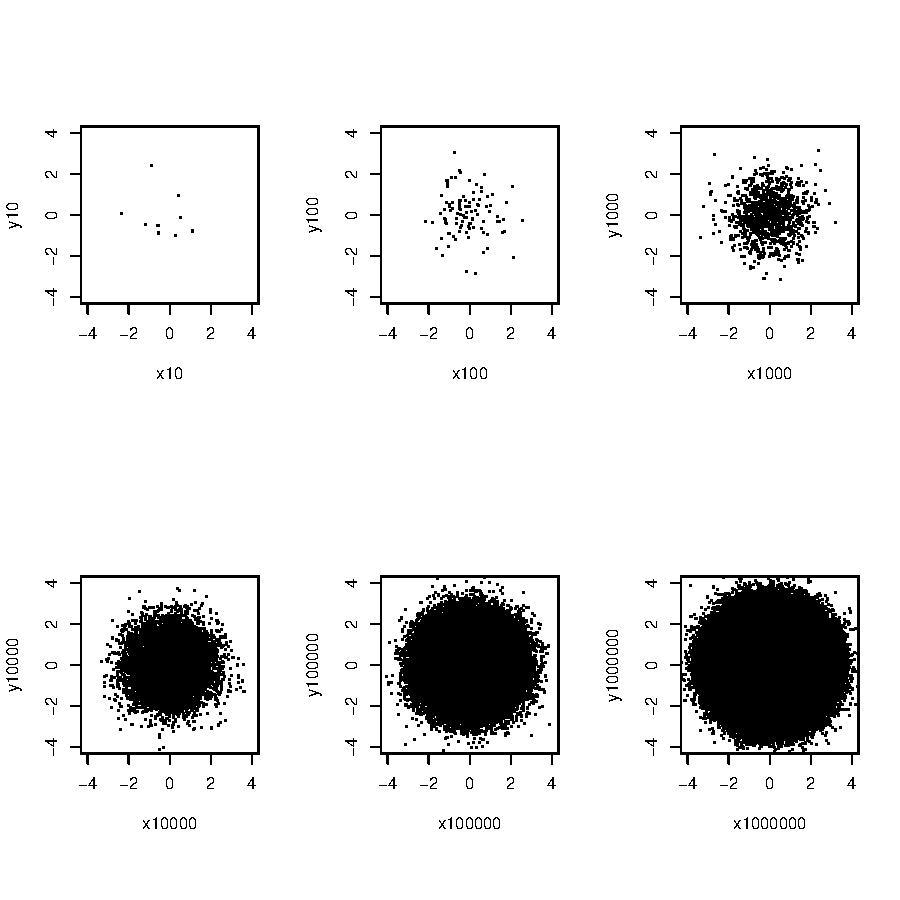
\includegraphics{lect_main-003}


\newpage


\subsection{Contour Plots and Bivariate Density Plots}


Several suggestions for baseR and ggplot were obtained at this web page:
\url{https://stats.stackexchange.com/questions/31726/scatterplot-with-contour-heat-overlay}

\begin{Schunk}
\begin{Sinput}
> library(MASS)
> # some pretty colors
> library(RColorBrewer)
> my.cols <- brewer.pal(9, "YlOrRd")
> par(mfrow = c(1, 2))
> # compute 2D kernel density, see MASS book, pp. 130-131
> z10000 <- kde2d(x10000, y10000, n = 50)
> z100000 <- kde2d(x100000, y100000, n = 50)
> plot(x10000, y10000, xlim = c(-4.0, 4.0), ylim = c(-4.0, 4.0),
+      xlab = "X label", ylab = "Y label", pch = 19, cex = 0.4)
> contour(z10000, drawlabels = FALSE, nlevels = 9, col = my.cols, add = TRUE, lwd = 5)
> plot(x100000, y100000, xlim = c(-4.0, 4.0), ylim = c(-4.0, 4.0),
+      xlab = "X label", ylab = "Y label", pch = 19, cex = 0.4)
> contour(z100000, drawlabels = FALSE, nlevels = 9, col = my.cols, add = TRUE, lwd = 5)
\end{Sinput}
\end{Schunk}
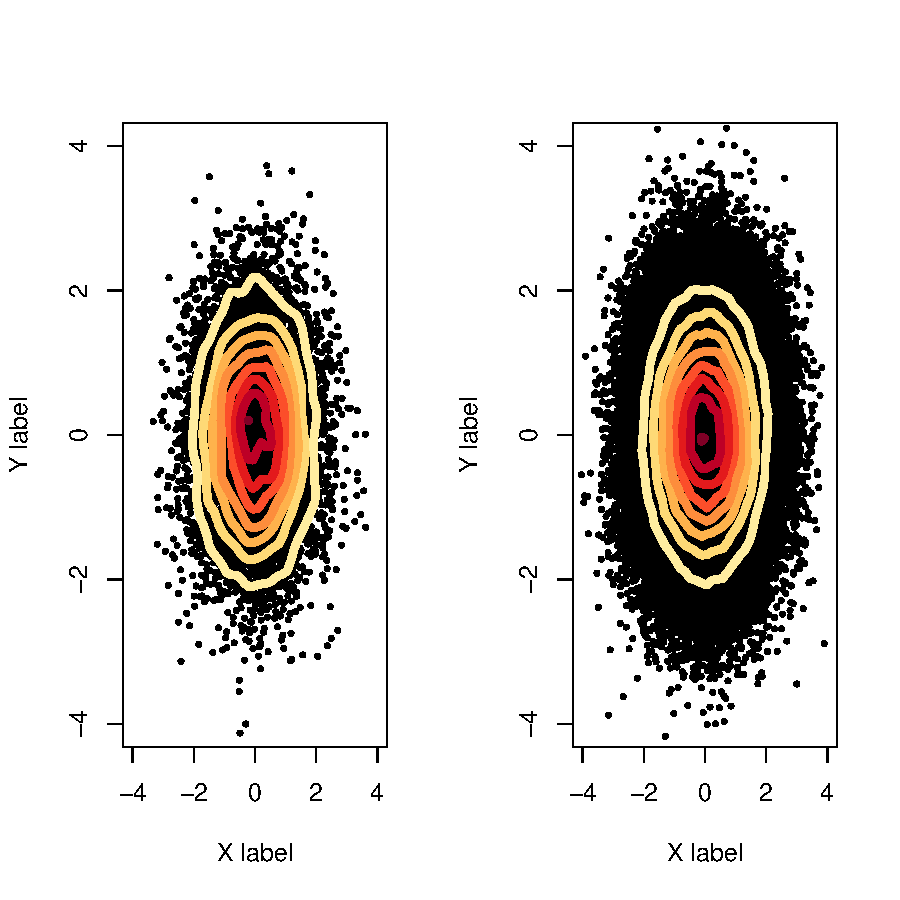
\includegraphics{lect_main-004}


\begin{Schunk}
\begin{Sinput}
> library(ggplot2)
> library(gridExtra)
> df10000 <- data.frame(x = x10000, y = y10000)
> commonTheme <- list(labs(color = "Density",
+                          fill = "Density",
+                          x = "X label",
+                          y = "Y label"),
+                     theme_bw(),
+                     theme(legend.position = c(0.02, 0.98),
+                           legend.justification = c(0, 1)))
> g1 <- ggplot(data = df10000, aes(x, y)) + 
+   xlim(-4, 4) +
+   ylim(-4, 4) +
+   geom_point() +
+   geom_density2d(aes(colour = ..level..)) + 
+   scale_colour_gradient(low = "yellow", high = "red") + 
+   commonTheme
> g1
\end{Sinput}
\end{Schunk}


\begin{Schunk}
\begin{Sinput}
> g2 <- ggplot(data = df10000, aes(x, y)) + 
+   xlim(-4, 4) +
+   ylim(-4, 4) +
+   geom_point() +
+   scale_fill_continuous(low = "yellow", high = "red") +
+   stat_density2d(aes(fill = ..level.., alpha = ..level..), geom = "polygon", colour = "black") + 
+   guides(alpha = "none") +
+   commonTheme
> g2
\end{Sinput}
\end{Schunk}


\begin{Schunk}
\begin{Sinput}
> g3 <- ggplot(data = df10000, aes(x, y)) + 
+   xlim(-4, 4) +
+   ylim(-4, 4) +
+   stat_density_2d(geom = "point", aes(size = ..density..), n = 20, contour = FALSE) + 
+   guides(alpha = "none") +
+   commonTheme
> g3
\end{Sinput}
\end{Schunk}


\begin{Schunk}
\begin{Sinput}
> grid.arrange(g1, g2, g3, nrow = 2)
\end{Sinput}
\end{Schunk}
\includegraphics{lect_main-008}


\newpage


\subsection{Hexagon Binning}


{\bf (Based on \cite{CLNL87})}


The R help page for hexbin indicates:
\begin{quotation}
``Creates a ``hexbin'' object. Basic components are a cell id and a count of 
points falling in each occupied cell.''
\end{quotation}

Let us apply hexbin to data from our bivariate normal distribution
for 10,000 and 1,000,000 observations.

\underline{\bf Example 3:}
%
\begin{Schunk}
\begin{Sinput}
> library(hexbin)
> library(colorspace)
> plot(hexbin(x10000, y10000))
\end{Sinput}
\end{Schunk}
\includegraphics{lect_main-009}

\begin{Schunk}
\begin{Sinput}
> plot(hexbin(x10000, y10000), colramp = heat.colors)
\end{Sinput}
\end{Schunk}
\includegraphics{lect_main-010}

\begin{Schunk}
\begin{Sinput}
> plot(hexbin(x10000, y10000), style = "lattice")
\end{Sinput}
\end{Schunk}
\includegraphics{lect_main-011}

\begin{Schunk}
\begin{Sinput}
> plot(hexbin(x10000, y10000), style = "centroid")
\end{Sinput}
\end{Schunk}
\includegraphics{lect_main-012}

\begin{Schunk}
\begin{Sinput}
> plot(hexbin(x10000, y10000), colramp = terrain.colors)
\end{Sinput}
\end{Schunk}
\includegraphics{lect_main-013}

\begin{Schunk}
\begin{Sinput}
> plot(hexbin(x10000, y10000, xbins = 16), colramp = topo.colors)
\end{Sinput}
\end{Schunk}
\includegraphics{lect_main-014}


Hexagonal binning in ggplot2:

\begin{Schunk}
\begin{Sinput}
> library(ggplot2)
> library(gridExtra)
> g1 <- ggplot(data = df10000, aes(x, y)) + 
+   xlim(-4, 4) +
+   ylim(-4, 4) +
+   geom_hex() 
> g1
\end{Sinput}
\end{Schunk}


\begin{Schunk}
\begin{Sinput}
> g2 <- ggplot(data = df10000, aes(x, y)) + 
+   xlim(-4, 4) +
+   ylim(-4, 4) +
+   geom_hex(binwidth = c(0.5, 0.5)) 
> g2
\end{Sinput}
\end{Schunk}


\begin{Schunk}
\begin{Sinput}
> grid.arrange(g1, g2, nrow = 2)
\end{Sinput}
\end{Schunk}
\includegraphics{lect_main-017}


\newpage


\subsection{Bivariate Histograms}


Execute this code once to create the bivhist3d function,
written by Mike Minnotte:
%
{\scriptsize
\begin{Schunk}
\begin{Sinput}
> bivhist3d <- function(x, y, nbins = nclass.Sturges(x), 
+                       col = c(heat.colors(19)), xlab = "x", ylab = "y")
+   
+   # Bivariate histogram plot.  Uses the gplots and rgl libraries.
+   # Written by Mike Minnotte
+ {
+   h2d <- hist2d(x, y, nbins, show = FALSE)
+   xb <- h2d$x
+   yb <- h2d$y
+   count <- h2d$counts
+   xs <- (xb[2] - xb[1]) / 2
+   ys <- (yb[2] - yb[1]) / 2
+   xb <- xb + xs
+   yb <- yb + ys
+   
+   if (length(col) > 1)
+     zcol <- matrix(cut(count, length(col), labels = FALSE), length(xb))
+   else 
+     zcol <- matrix(1, length(xb), length(yb))
+   
+   cube <- cube3d()
+   clear3d()
+   bg3d(col = "grey")
+   
+   xr <- max(xb) - min(xb)
+   yr <- max(yb) - min(yb)
+   zr <- max(count)
+   mr <- max(xr, yr, zr) * 0.8
+   
+   aspect3d(mr / xr, mr / yr, mr / zr)
+   
+   for (i in 1:length(xb)) 
+     for (j in 1:length(yb))
+     {
+       scube <- scale3d(cube, xs, ys, count[i, j] / 2)
+       tcube <- translate3d(scube, xb[i], yb[j], count[i, j] / 2)
+       if (count[i, j] == 0) 
+         shade3d(tcube, color = "black")
+       else 
+         shade3d(tcube, color = col[zcol[i, j]])
+     }
+   
+   axes3d()
+   title3d(xlab = xlab, ylab = ylab, zlab = "count")
+   return()
+ }
\end{Sinput}
\end{Schunk}
}


\newpage


Let us apply bivhist3d to data from our bivariate normal distribution
for 10,000 observations.
%
\begin{Schunk}
\begin{Sinput}
> library(gplots)
> library(rgl)
> bivhist3d(x10000, y10000)
\end{Sinput}
\begin{Soutput}
NULL
\end{Soutput}
\begin{Sinput}
> bivhist3d(x10000, y10000, col = "red")
\end{Sinput}
\begin{Soutput}
NULL
\end{Soutput}
\begin{Sinput}
> bivhist3d(x10000, y10000, col = terrain.colors(15), nbins = 20)
\end{Sinput}
\begin{Soutput}
NULL
\end{Soutput}
\end{Schunk}


If you want to create a snapshot of an interesting 3D view,
use the command:
%
\begin{Schunk}
\begin{Sinput}
> #rgl.snapshot("bivhist1.png")
\end{Sinput}
\end{Schunk}


Finally, let us do some automatic animation, based on 
\url{https://stat.ethz.ch/pipermail/r-devel/2014-April/068817.html}:


\begin{Schunk}
\begin{Sinput}
> bivhist3d(x10000, y10000, col = terrain.colors(15), nbins = 20)
\end{Sinput}
\begin{Soutput}
NULL
\end{Soutput}
\begin{Sinput}
> U <- par3d("userMatrix")
> for (theta in seq(0, 2 * pi, len = 100)) {
+    par3d(userMatrix = rotationMatrix(theta, 0, 1, 0) %*% U ) # Rotate about the z-axis
+    Sys.sleep(0.1)
+ }
\end{Sinput}
\end{Schunk}


\newpage


\subsection{Further Reading}

Additional sources for bivariate plots are:

\begin{itemize}

\item To be announced.

\end{itemize}


~\\[2cm]

\begin{figure}[ht]
\centering{\includegraphics[height=4in]{Scans//Cartoonstock_RoomBelow.png}}
\caption{\label{Cartoonstock_RoomBelow}
\url{http://www.cartoonstock.com/cartoonview.asp?start=4&search=main&catref=bven597&MA_Artist=&MA_Category=&ANDkeyword=statistics&ORkeyword=&TITLEkeyword=&NEGATIVEkeyword=},
Cartoon.
}
\end{figure}


\newpage


%\SweaveInput{lect_chapter7.Rnw}
%\SweaveInput{lect_chapter8.Rnw}
%\SweaveInput{lect_chapter3.Rnw}
%\SweaveInput{lect_chapter9.Rnw}
%\SweaveInput{lect_chapter10.Rnw}
%\SweaveInput{lect_chapter2.Rnw}


\setcounter{page}{1}
\addcontentsline{toc}{section}{References}

\bibliography{references}


\vspace*{1cm}

\centering{\bf \LARGE --- THE END ---}~\\[1cm]

\begin{figure}[ht]
\centering{\includegraphics[height=3in]{Scans//Cartoonstock_FallingArrow.jpg}}
\caption{\label{Cartoonstock_FallingArrow}
\url{http://www.cartoonstock.com/blowup_stock.asp?imageref=vsh0184&artist=Shirvanian,+Vahan&topic=statistics+}, 
Cartoon.
}
\end{figure}


\end{document}

